\begin{frame}[label=zoverview]
    \frametitle{Zephyr Meteor Radar Network}
    \begin{columns}
        \begin{column}{0.6\textwidth}
            The \alert{Zephyr meteor radar network} is our lab's multistatic network, established late 2021.
            \begin{itemize}
                \item \(1\times\) interferometric \textcolor{blue}{\textbf{TX}} array in Boulder, CO
                \item \(4 \times\) \textcolor{red}{\textbf{RX}} throughout CO
                \item Fully polarimetric links
            \end{itemize}
        \end{column}
        \begin{column}{0.25\textwidth}
            \centering %
            {\linespread{1}\tiny %
            \centering%
            \begin{tabular}{R{1.5cm} m{1.1cm}}
                \hline
                \rowcolor[HTML]{C0C0C0} 
                \textbf{Parameter}                   & \textbf{Value}         \\ \hline
                Frequency:                   & 31.25 MHz     \\
                \textcolor{blue}{\textbf{TX}} bandwidth: & 200 kHz       \\
                Channel power:               & 500 W         \\
                Channels:             & 6             \\
                Code length:                 & 1,000 Chips   \\
                Chip duration:               & 5 \(\mu s\)   \\
                Chip length:            & 1.5 km  \\
                \hline
            \end{tabular}}%
        \end{column}
        \begin{column}{0.22\textwidth}
            \centering
            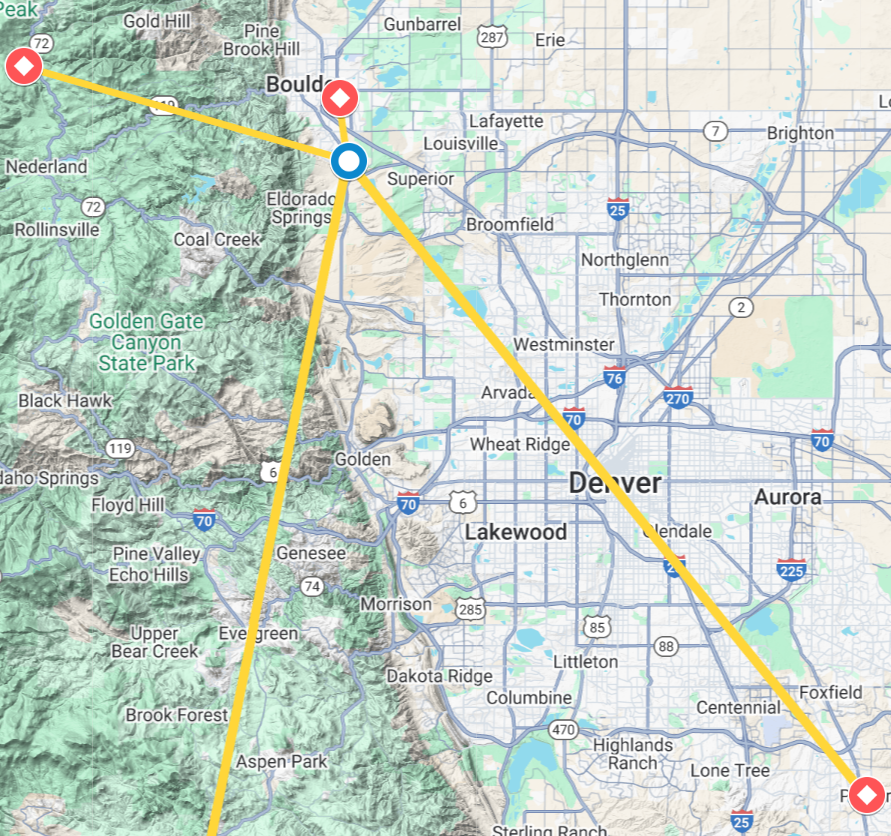
\includegraphics[width=\linewidth]{img/zephyr_map.png}
        \end{column}%
    \end{columns}%
    \centering
    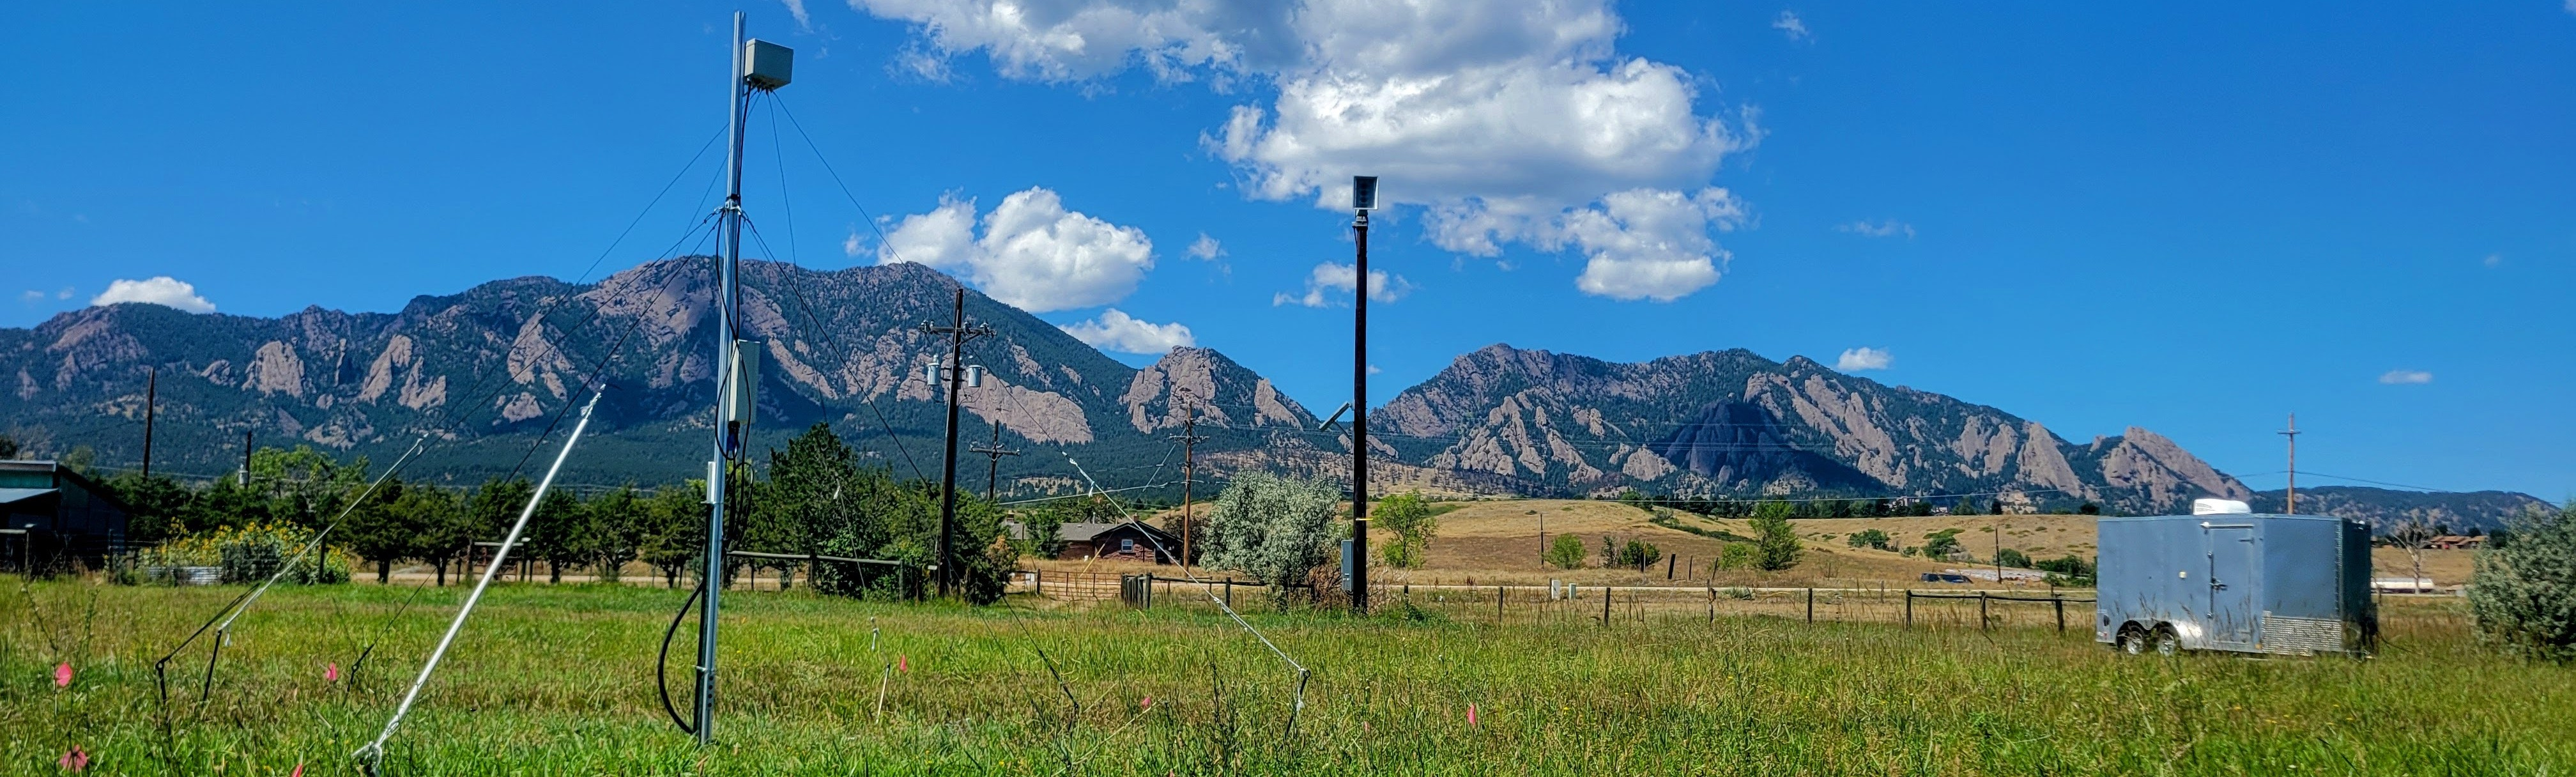
\includegraphics[width=\linewidth]{img/zephyr.jpg}
\end{frame}
